\chapter{Panoramica dell'applicazione web da dispositivo mobile}

In questo capitolo verrà effettuata una panoramica di come si presenta l'applicazione web da un dispositivo mobile.
\newline

\section{Dispositivo}
Il dispositivo utilizzato per la navigazione sulla web app realizzata è un dispositivo Apple, precisamente un iPhone che ha come sistema operativo iOS. \newline
Il browser utilizzato è Safari che risponde perfettamente a tutte le funzionalità dell'applicazione web.
\subsection{Set Up del Dispositivo}
Per far si che l'applicazione funzioni correttamente sono necessarie determinate impostazioni che sono elencate di seguito.
\begin{itemize}
\item Aprendo le impostazioni, andando sulla sezione privacy e aprendo la voce \textbf{Localizzazione} è possibile attivare il servizio di localizzazione del dispositivo;

\begin{figure}[H]
	\centering
	\caption{Impostazione che permette tramite spunta di abilitare l'opzione di localizzazione}
	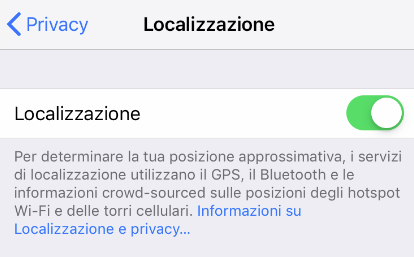
\includegraphics[]{abilita_gps.png}
\end{figure} 

\item Sempre nella stessa sezione si danno i permessi all'applicazione Safari di utilizzare tale servizio;

\begin{figure}[H]
	\centering
	\caption{Impostazione che permette tramite spunta di selezionare la voce Mentre si usa l'app}
	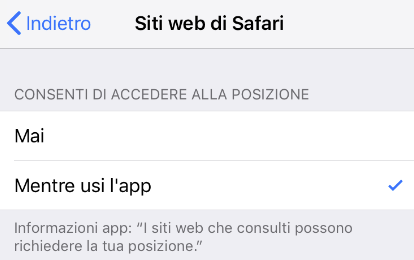
\includegraphics[]{safari_gps1.png}
\end{figure} 

\begin{figure}[H]
	\centering
	\caption{Dimostrazione della corretta procedura, Safari ha ora ottenuto i permessi}
	
\includegraphics[]{safari_gps2.png}
\end{figure} 


\item Sempre dalle impostazioni del dispositivo, selezionando safari è possibile abilitare l'utilizzo della fotocamera spuntando la relativa voce. (Questo passaggio è essenziale affinché nel front-end basic funzioni la parte per scattare una foto);
\begin{figure}[h]
	\centering
	\caption{Impostazioni che permettono tramite spunta delle voci 'Microfono e Fotocamera', di abilitare tali servizi}
	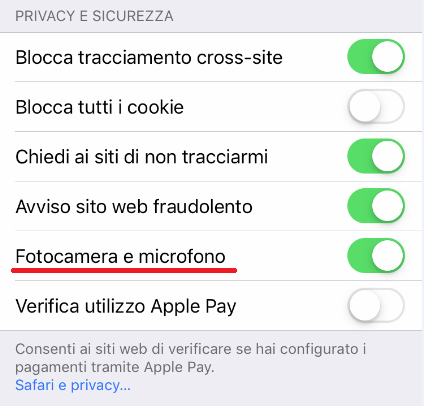
\includegraphics[scale=0.8]{fotocamera_safari.png}
\end{figure} 
\item Aprire l'ultima voce della sezione di Safari (Avanzate) e abilitare la voce \textbf{JavaScript};
\begin{figure}[h]
	\centering
	\caption{Impostazione che permette tramite spunta di abilitare le funzionalità 'JavaScript'}
	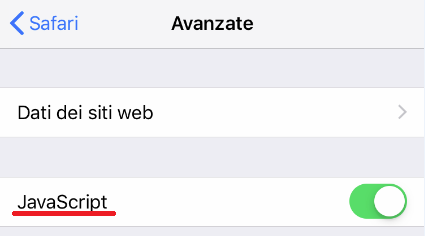
\includegraphics[scale=0.8]{safari_javascript.png}
\end{figure} 

\item A questo punto il dispositivo è settato correttamente e per accedere al sito si deve utilizzare il protocollo \textbf{HTTPS} e non il protocollo HTTP (altrimenti le API non funzionerebbero).

\end{itemize}

\section{Navigazione dell'applicazione Web}

\subsection{Full Front-End}
\subsubsection{Richiesta di Localizzazione}
\begin{figure}[H]
	\centering
	\caption{Richiesta di Localizzazione da parte dell'API, accettando si acconsente a condividere la proprio posizione affinché l'applicazione web funzioni correttamente.}
	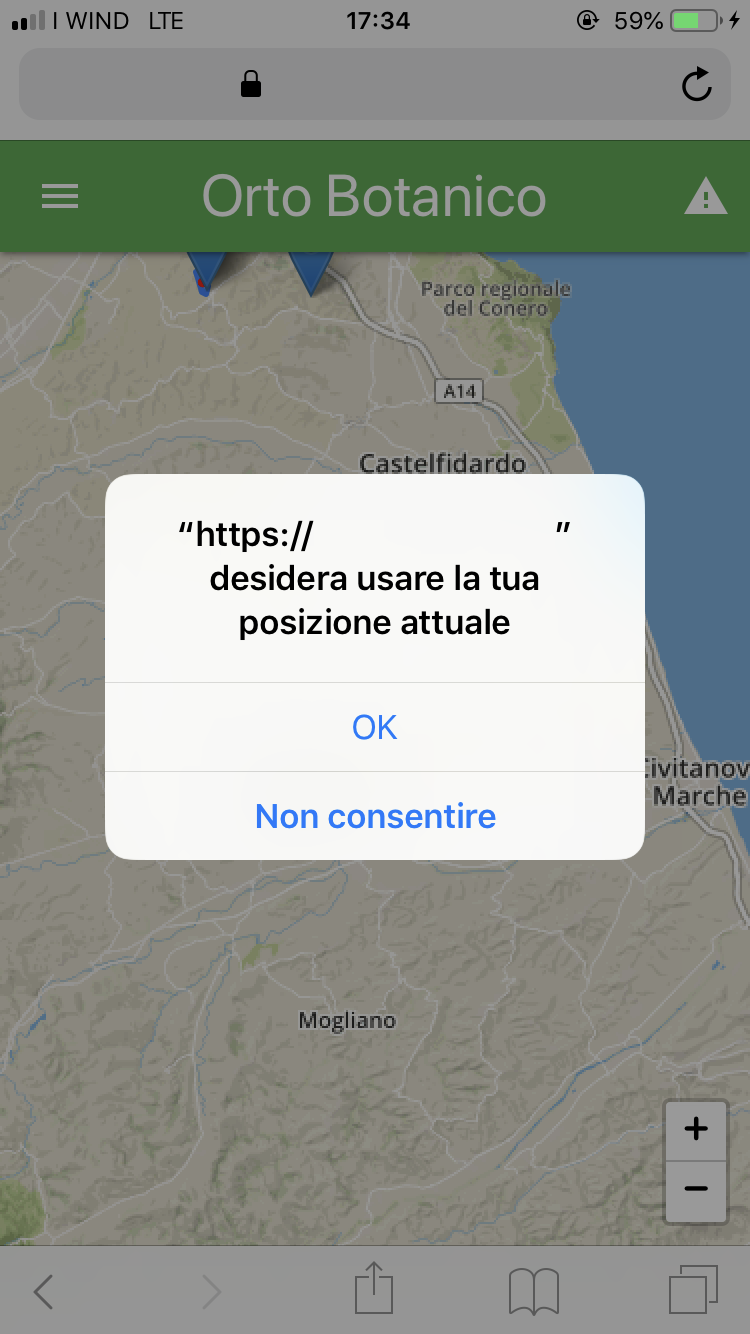
\includegraphics[scale=0.3]{location_request.png}
\end{figure} 
\newpage
\subsubsection{Homepage}
\begin{figure}[H]
	\centering
	\caption{Come si presenta l'homepage dell'applicazione Web con il front end full} 
	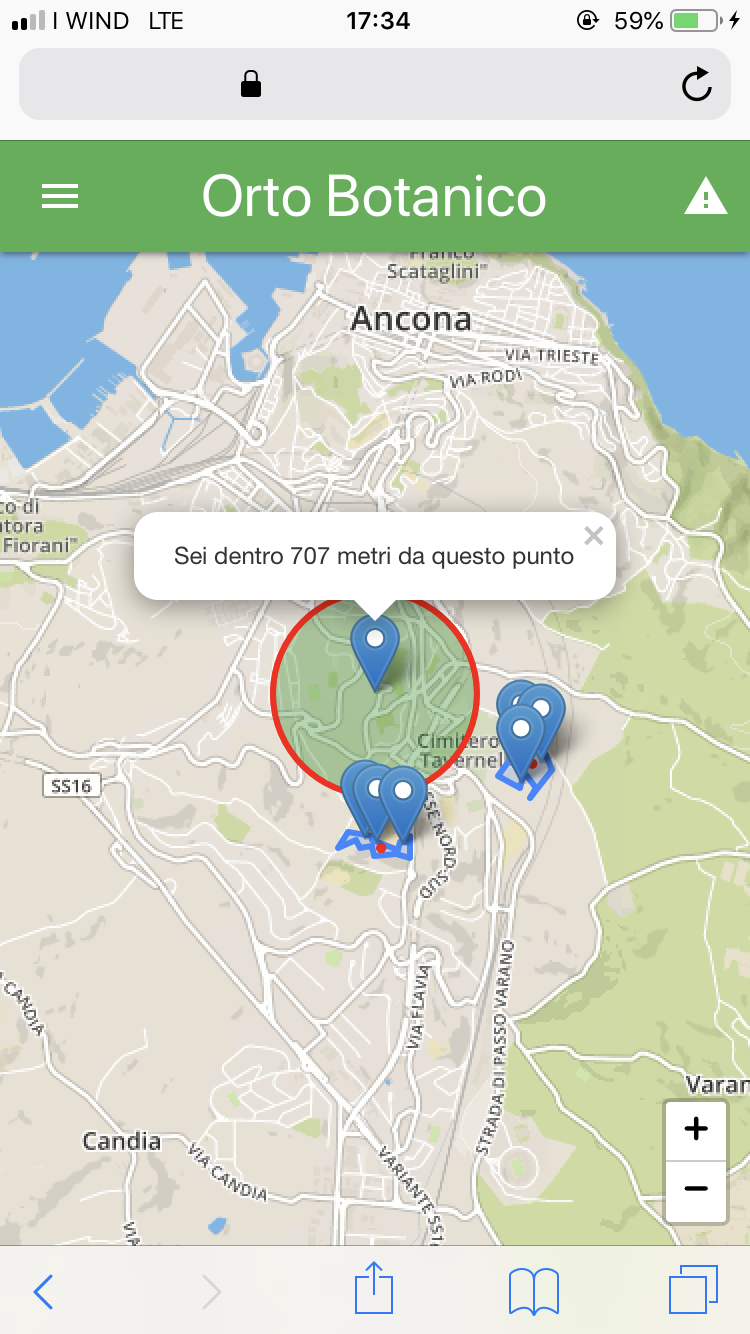
\includegraphics[scale=0.3]{homepage.png}
\end{figure} 
\newpage

\subsubsection{Sidebar}
\begin{figure}[H]
	\centering
	\caption{Come si presenta la sidebar di questo front end}
	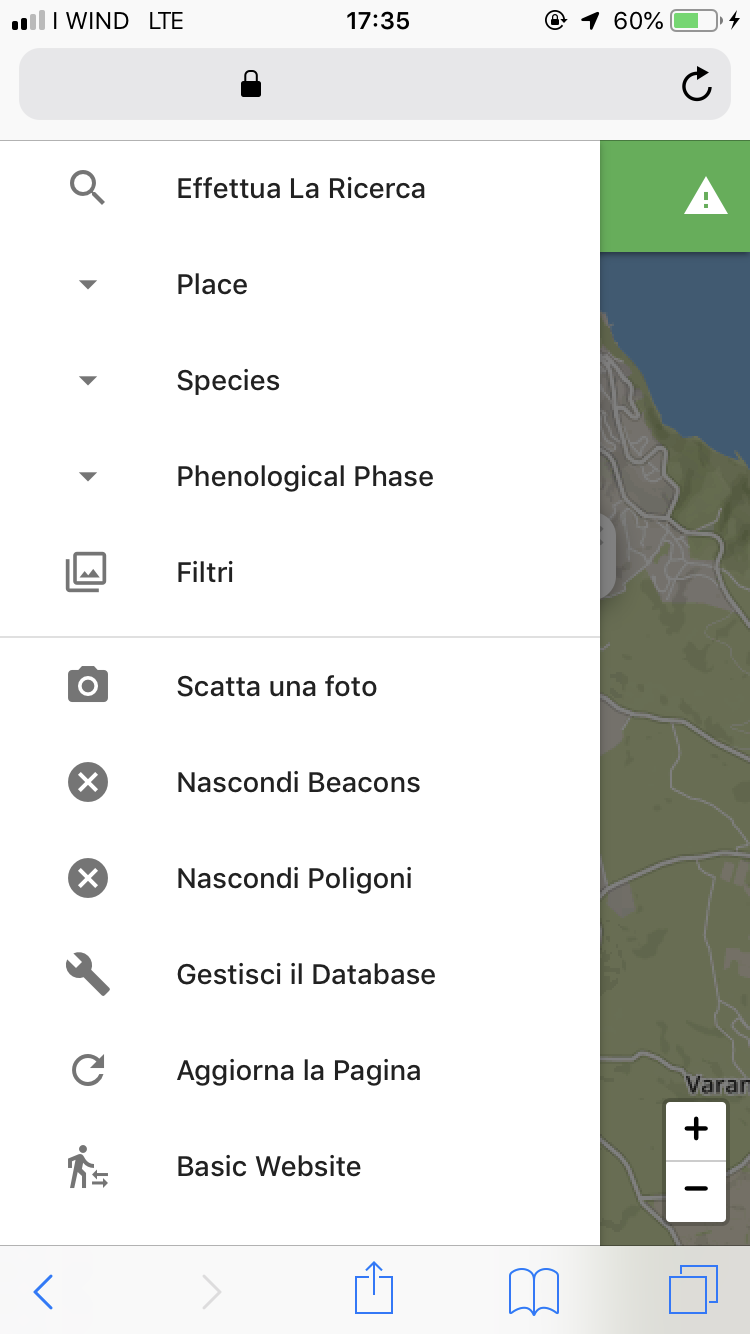
\includegraphics[scale=0.3]{sidebar.png}
\end{figure} 
\newpage

\subsubsection{Form Modale al click del Beacon}
\begin{figure}[H]
	\centering
	\caption{Ecco come si presenta la form che viene mostrata al click del beacon sulla mappa}
	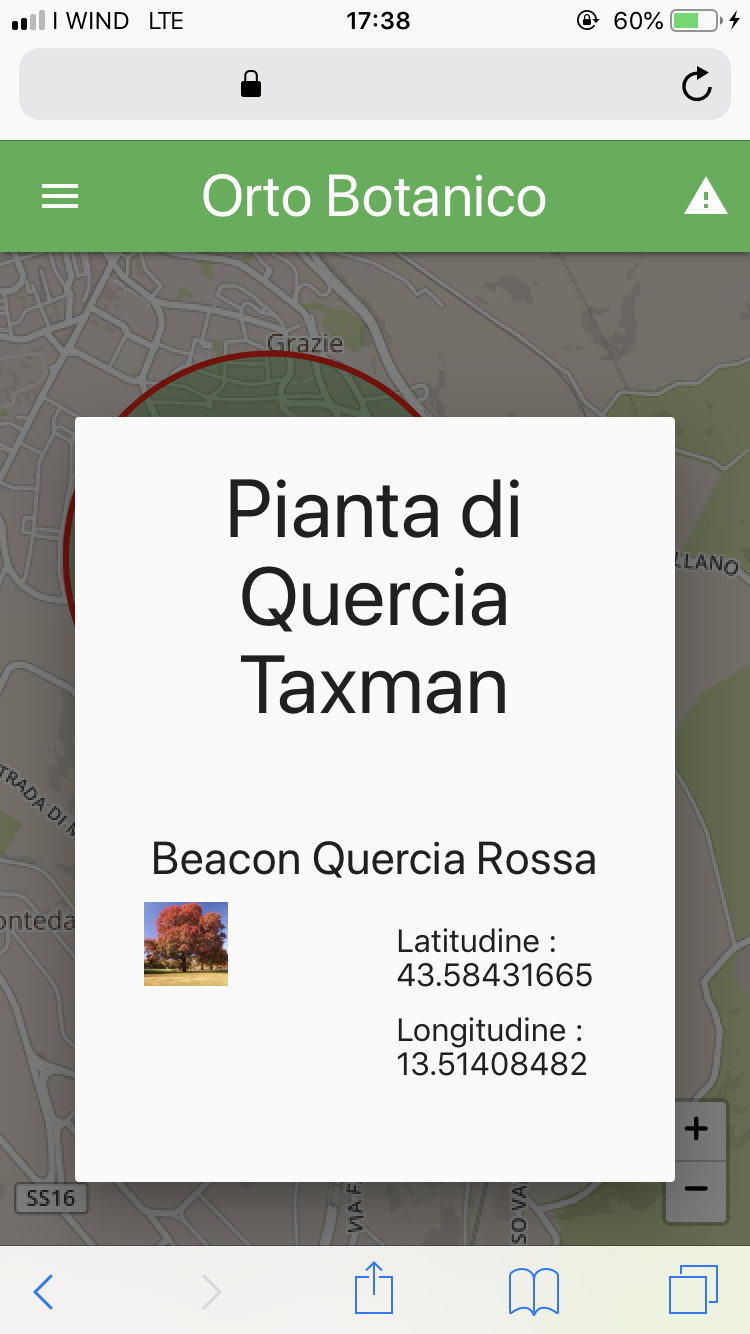
\includegraphics[scale=0.3]{beacon_popup.png}
\end{figure} 
\newpage

\subsubsection{Material Box della Form Modale del Beacon}
\begin{figure}[h]
	\centering
	\caption{Ecco come si presenta la Material Box (Light Box) al click dell'immagine della finestra modale del beacon}
	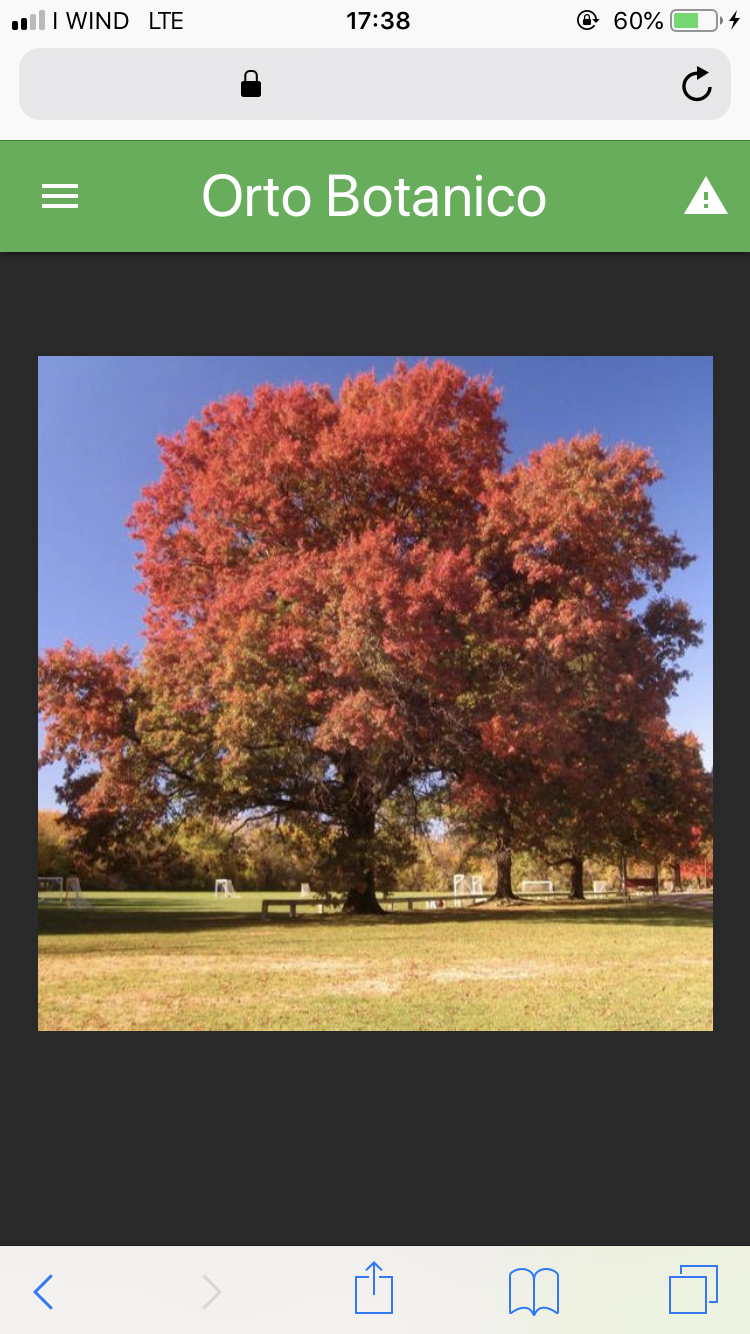
\includegraphics[scale=0.3]{material_box.png}
\end{figure} 
\newpage


\subsection{Basic Front-End}

\subsubsection{Homepage}
\begin{figure}[h]
	\centering
	\caption{Come si presenta l'homepage dell'applicazione Web con il front end basic}
	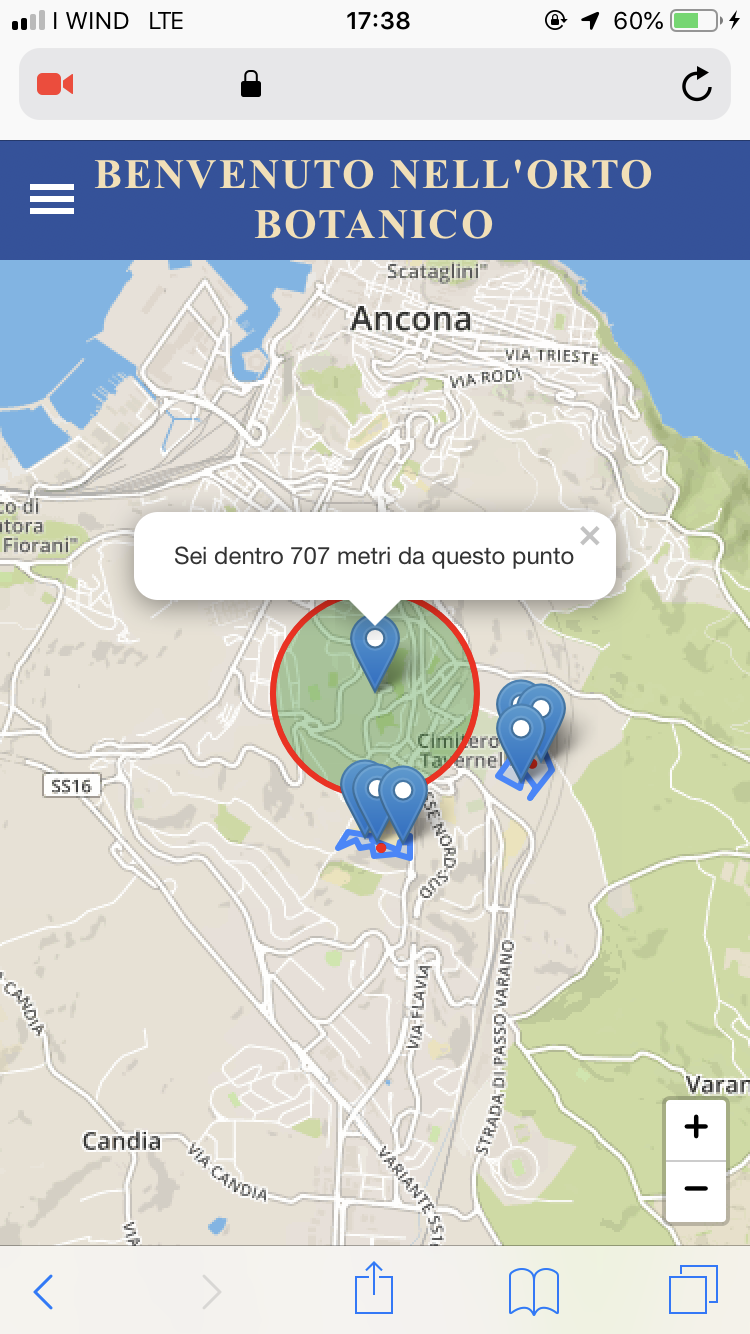
\includegraphics[scale=0.3]{homepage_basic.png}
\end{figure} 
\newpage

\subsubsection{Sidebar}
\begin{figure}[h]
	\centering
	\caption{Come si presenta la sidebar di questo front end}
	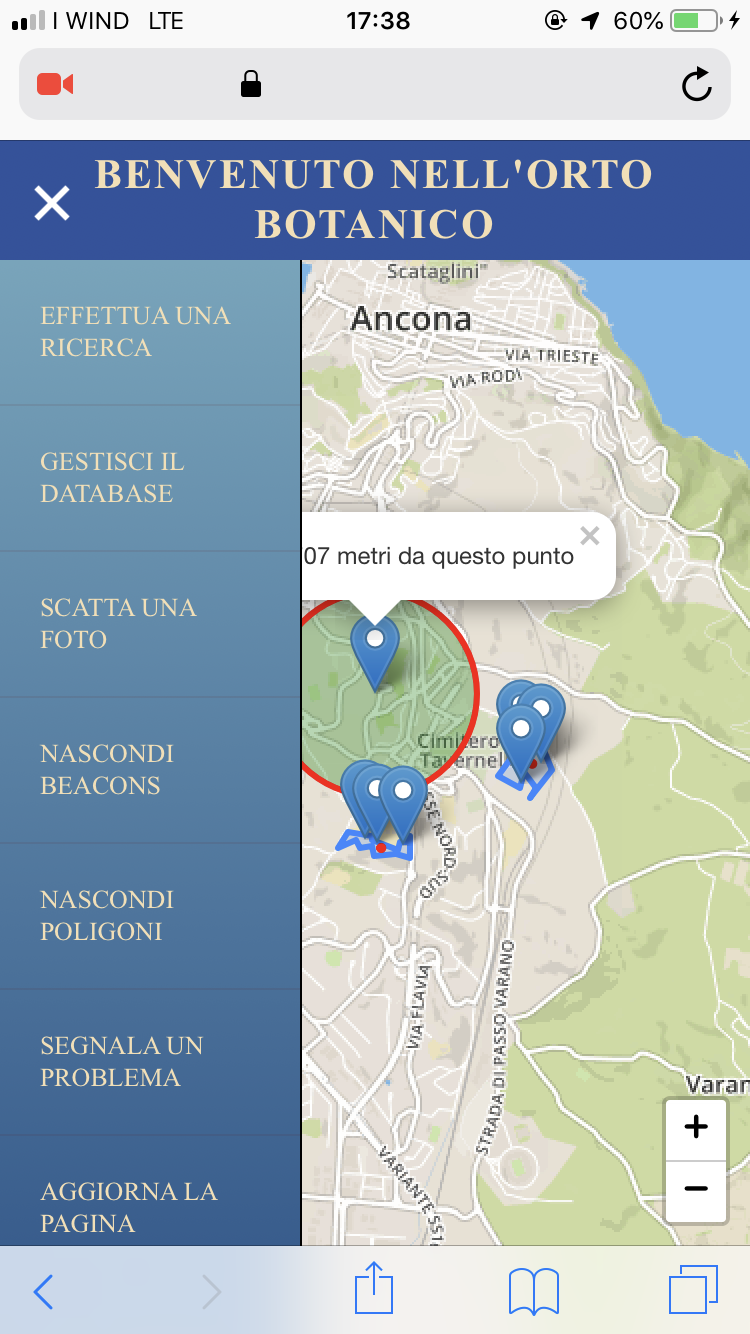
\includegraphics[scale=0.3]{sidebar_basic.png}
\end{figure} 
\newpage

\subsubsection{Finestra Modale per scattare Foto}
\begin{figure}[h]
	\centering
	\caption{Come si presenta la form modale per scattare le foto.}
	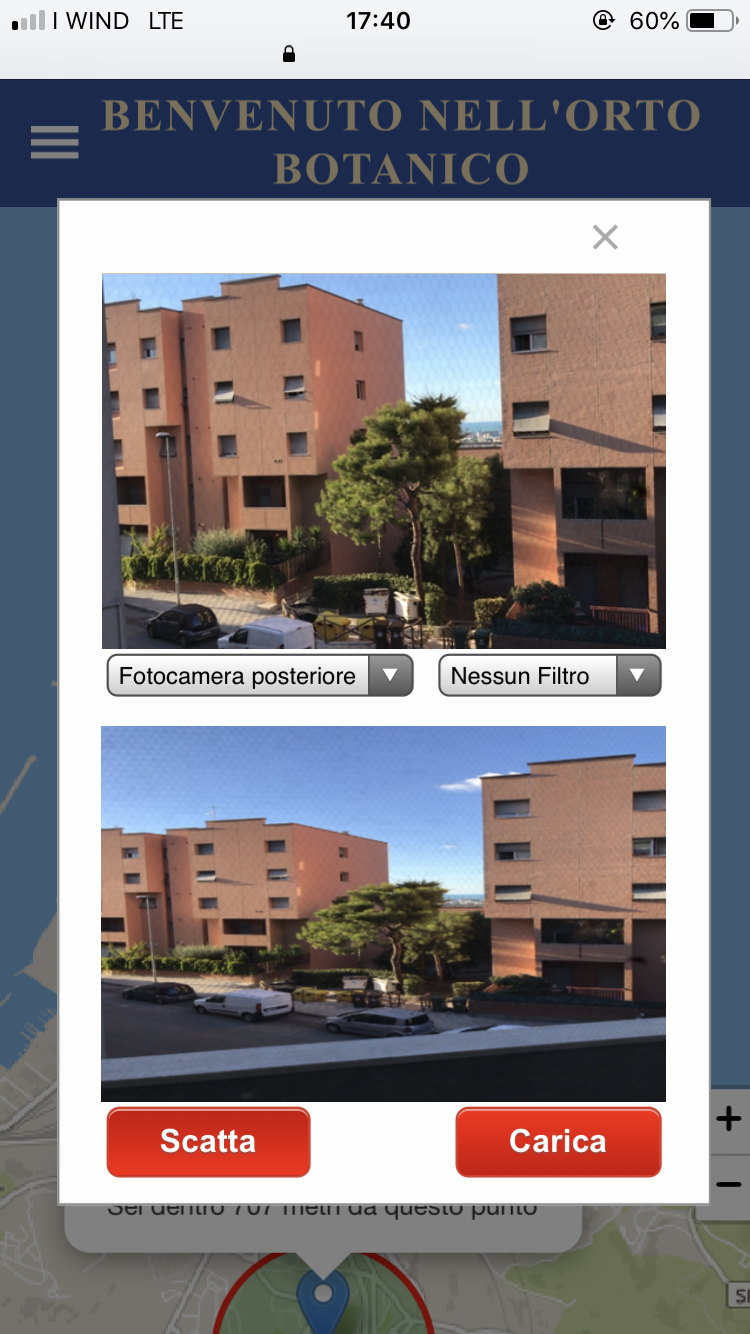
\includegraphics[scale=0.3]{canvas.png}
\end{figure} 
\newpage

